\newpage
\section{Introduction}
% Context and motivation
% Problem statement
% Project objectives
% Brief overview of existing solutions/literature review
% Brief introduction to energy investment optimization and the need for automated analysis tools.

\subsection{Project Context}
Energy systems are increasingly critical in modern society due to rising electricity demand and the global push toward 
cleaner energy sources. Power flow studies, which evaluate how electricity moves through transmission networks, identify
optimal generation mixes, ensure technical feasibility and able to optimize the location of assets. 

% \begin{figure}[h]
%     \centering
%     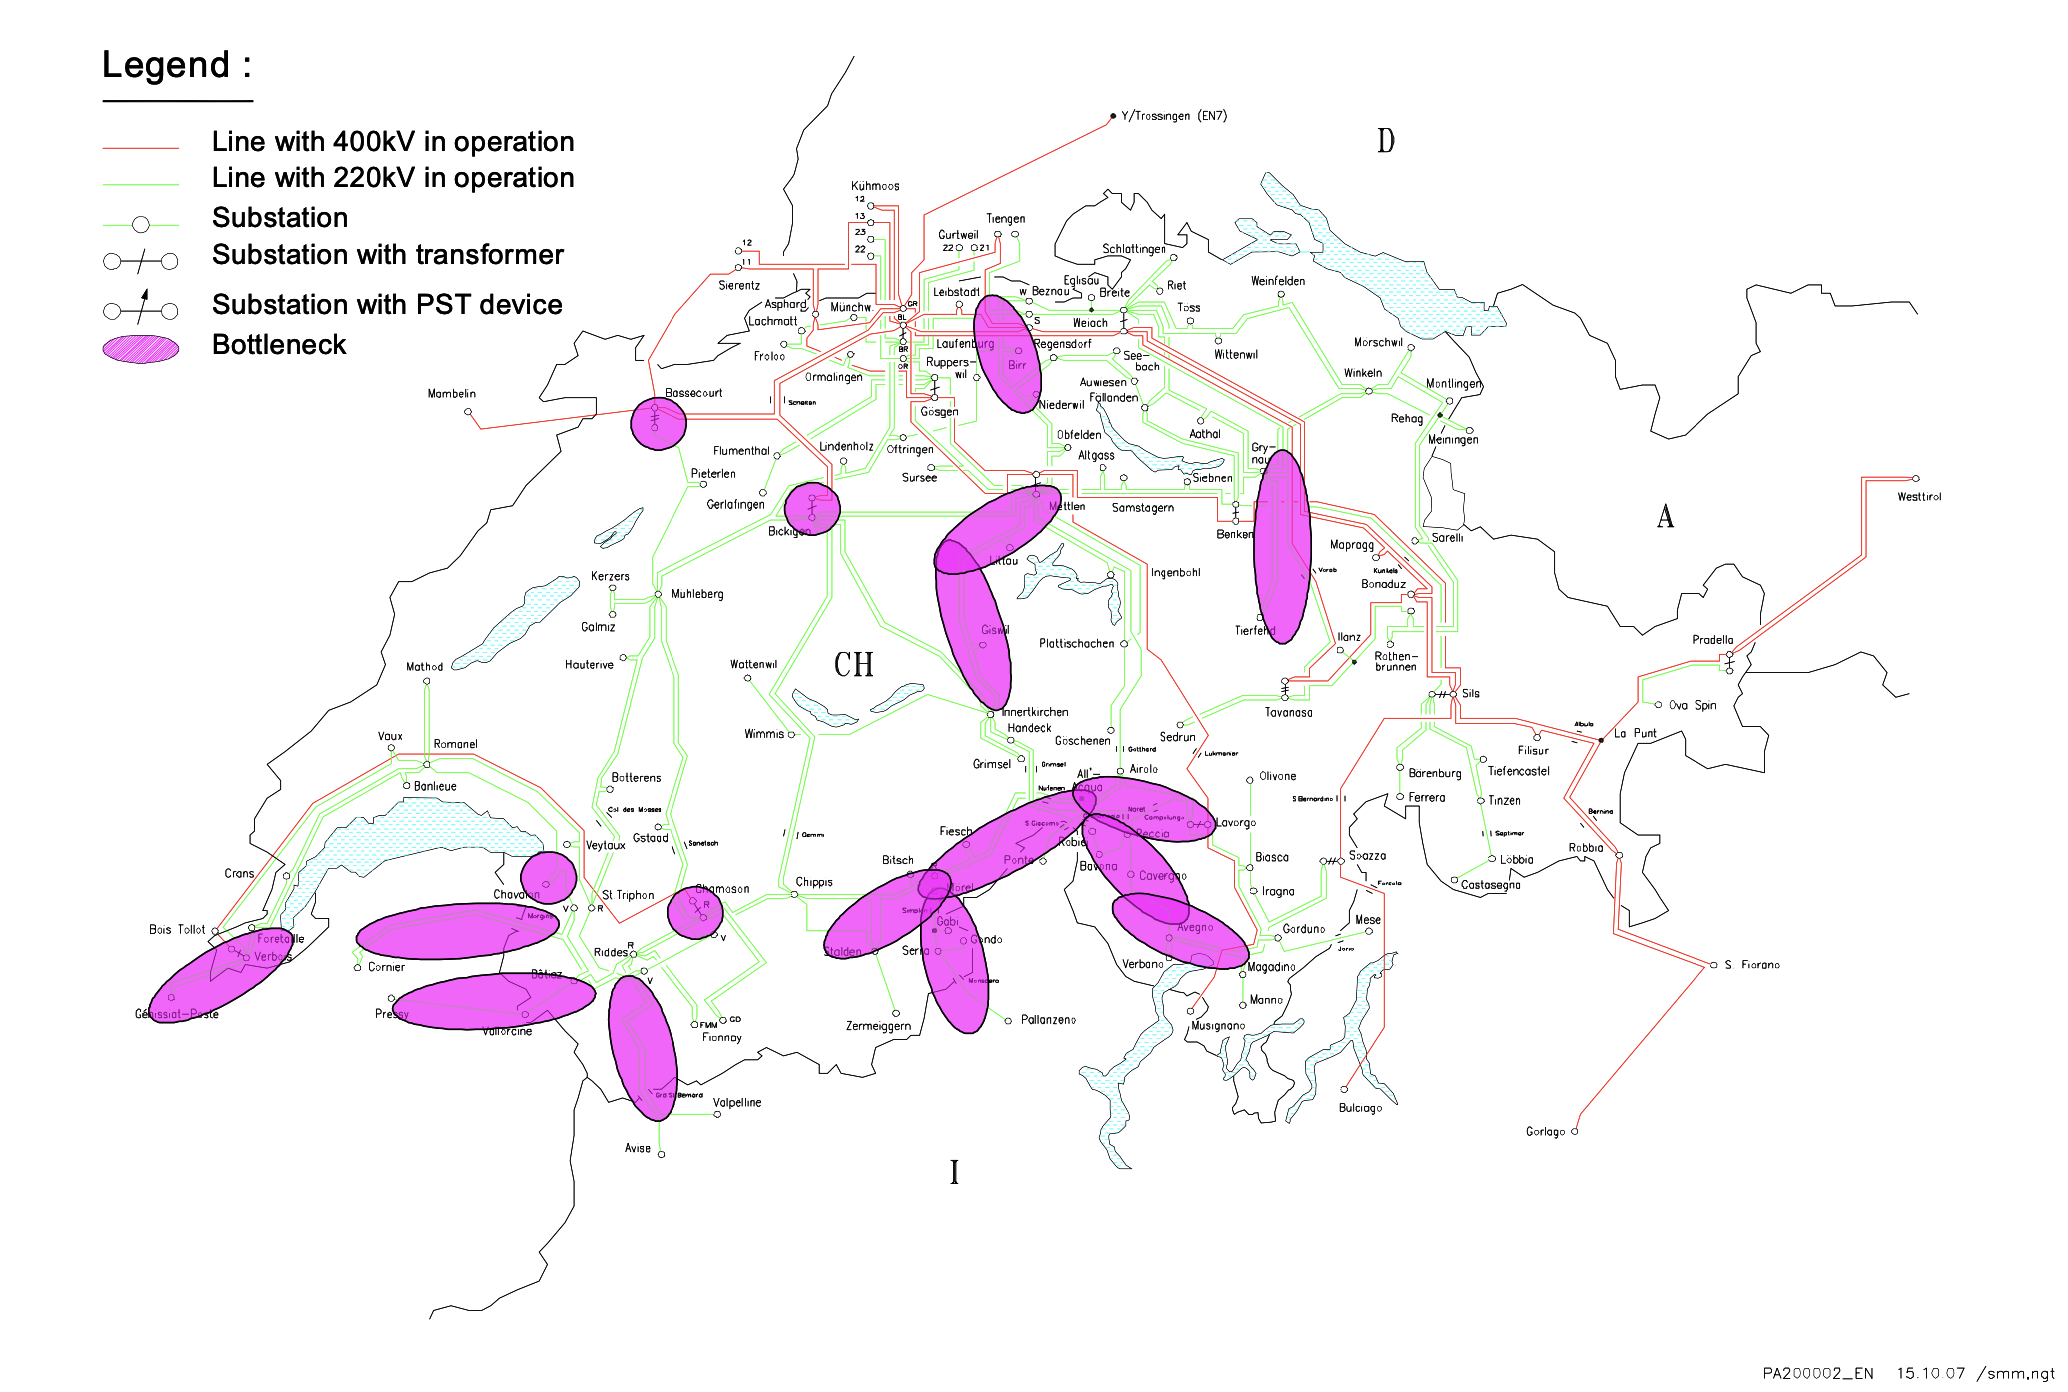
\includegraphics[width=0.5\textwidth]{images/bottlenecks-high-voltage.png}
%     \caption{Example of bottlenecks in the high-voltage transmission grid for general supply~\cite{swiss_infrastructure_2010}}
% \end{figure}

In addition to analyzing power flows, it incorporates financial metrics and the analysis of various generation assets, 
including renewables and storage ones. It underscores the ongoing importance of power flow problems in both daily grid 
operations and strategic energy planning.

Undertaken as a semester project (so-called specialisation project) for the MSE program, it builds mainly on methodologies 
from life cycle management and optimization~\cite{optimization_notes} courseworks. The project offers a reproducible 
demonstration of how technical and economic feasibility can be linked.


%---------------------------------------------------------------------------------------
\subsection{Objectives}
The project sets three main objectives:
\begin{enumerate}
    \item Develop a DC Optimal Power Flow (DCOPF) solver capable of handling multi-scenario analyses with variable 
    generation and storage configurations.
    \item Implement an investment analysis approach
    \item Demonstrate a comparative method for evaluating different resource mixes under diverse load profiles and cost 
    assumptions.
\end{enumerate}

The main challenge here is to compare multiple generation and storage configurations within an existing electrical grid. 
On the technical side, a \emph{DC power flow} is formulated and solved via linear programming, yielding hourly dispatch 
decisions under network constraints. While various objective functions could be considered—such as emissions reduction—this 
implementation focuses solely on cost minimization, subject to physical network constraints.

For the economic dimension, we opted to implement an \emph{investment analysis} framework—focusing on Net Present 
Value (NPV), annuity, and a load-based sensitivity analysis to gauge long-term costs across different scenarios. This 
integrated perspective provides a structured way to identify cost-effective integration of renewable and storage assets.

\newpage 
